%!TEX root = ../thesis.tex

\vspace{-10pt}

\section{本章の概要}
本章では,\ref{sec:nav-sys}節でシステムの概要を示す.また,\ref{sec:real-robot}節で実ロボットにおける歩行者の位置計算の詳細,\ref{sec:nav-usage}節でナビゲーションにおける予測結果の利用方法について述べる.

\section{実験概要}
予測結果をナビゲーションに応用したシステムによって,移動ロボットの挙動がどのように変化するか観察し,評価するために実験を行う.実験では,2つのナビゲーションシナリオで移動ロボットを自律走行させてデータを取得した.

\section{実験方法}
実験の予測は,\ref{chap:proposed_method}章のネットワークを用いて行った.しかし,使用したモデルに関しては,ホールドアウト(Hold Out)方式で訓練を行った.それ以外は同様の学習条件である.
また,\ref{chap:application}章で述べたシステムを用いてナビゲーションに予測結果を応用している.

実験は\figref{Fig:sim-env}に示すような,Gazebo\cite{Gazebo62:online}のシミュレータ環境で行う.また,\figref{Fig:sim-robot}に示すように,シミュレータで再現した移動ロボット(ORNE-box2\cite{井口颯人2023屋外自律移動ロボットプラットフォーム-orne})を使用した.\figref{Fig:sim-actor}に示す歩行者は,Gazeboのプラグイン\cite{Actors-G87:online}を使用している.

\begin{figure}[H]
  \centering
 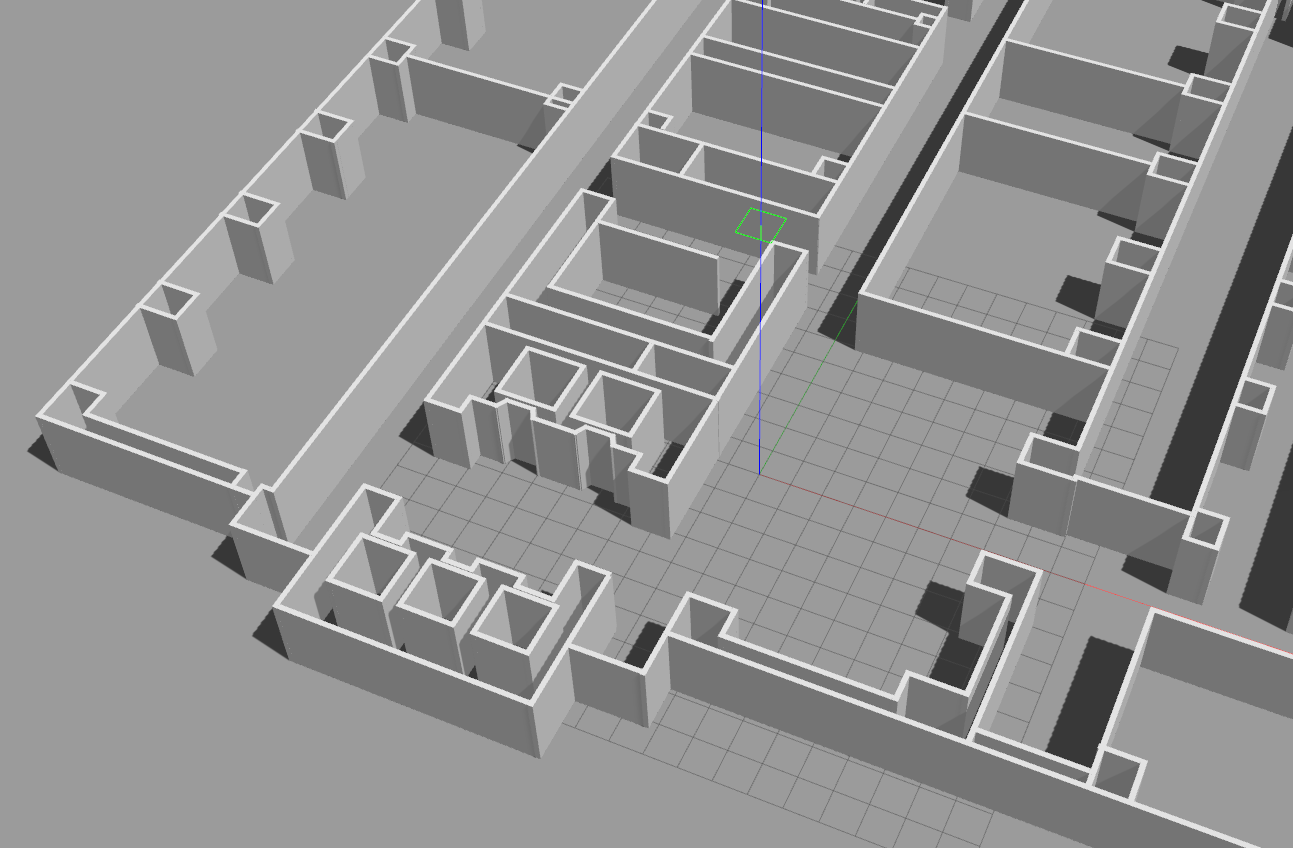
\includegraphics[keepaspectratio, scale=0.15]
      {images/sim-env.png}
\caption{Simulator Environment}
 \label{Fig:sim-env}
\end{figure} 

\vspace{-10pt}

\begin{figure}[H]
  \centering
  \begin{subfigure}{0.40\textwidth}
    \centering
    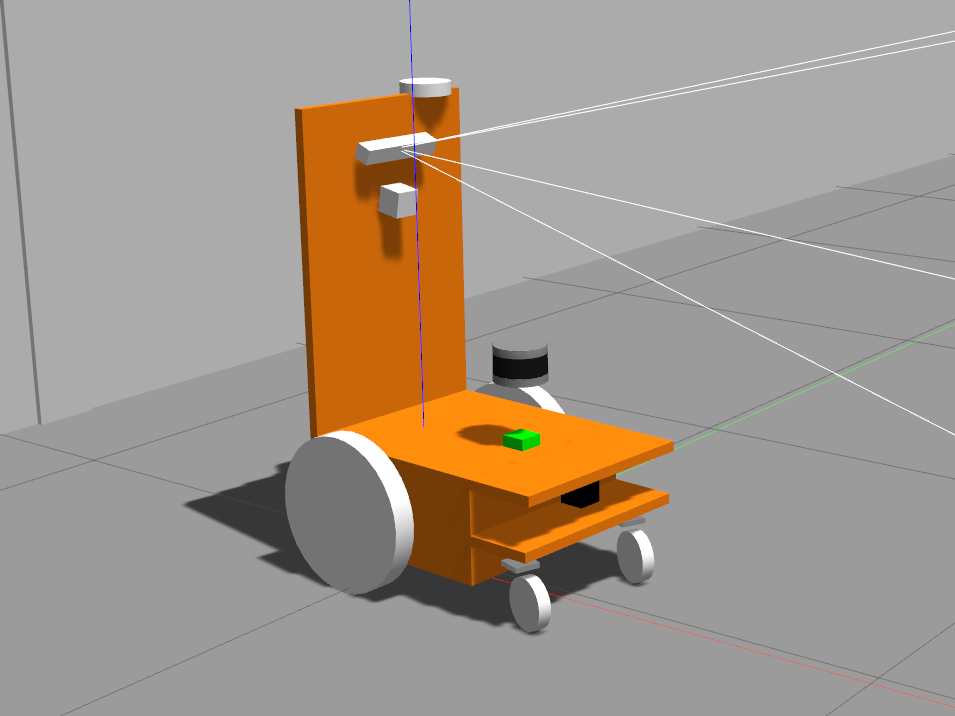
\includegraphics[keepaspectratio, scale=0.15]{images/sim-robot.png}
    \caption{Simulated Robot}
    \label{Fig:sim-robot}
  \end{subfigure}
  % \hfill
  \begin{subfigure}{0.40\textwidth}
    \centering
    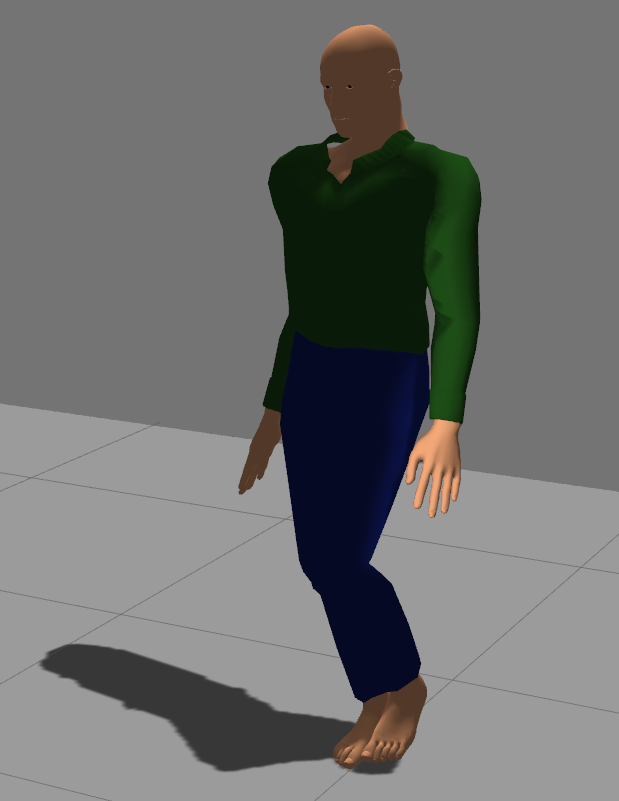
\includegraphics[keepaspectratio, scale=0.15]{images/sim-actor.png}
    \caption{Simulated Actor}
    \label{Fig:sim-actor}
  \end{subfigure}
  \caption{Simulated Robot and Actor}
  \label{Fig:sim-robot-actor}
\end{figure}

移動ロボットの自律走行は,つくばチャレンジ2024EX@イーアスつくば\cite{つくばチャレンジ36:online}で千葉工業大学 未来ロボティクス学科 box2チームが完走した際のソフトウェア構成,パラメータを参考にした.これは,Githubで公開されている\cite{openrdco85:online}.なお,シナリオには狭い通路の走行が含まれるため,並進速度やyaw方向の角速度は小さくなるように変更している.

\newpage

実験は\figref{Fig:experiment-scenarios}に示す2種類のシナリオで行った.
\figref{Fig:scenario1}に示すシナリオ1では,ロボットが直線経路を進む際に,歩行者が横断する状況を設定した.\figref{Fig:scenario2}に示すシナリオ2では,ロボットが狭い通路を進む際に,2名の歩行者がすれ違う状況を設定した.

\begin{figure}[H]
  \centering
  \begin{subfigure}{0.80\textwidth}
    \centering
    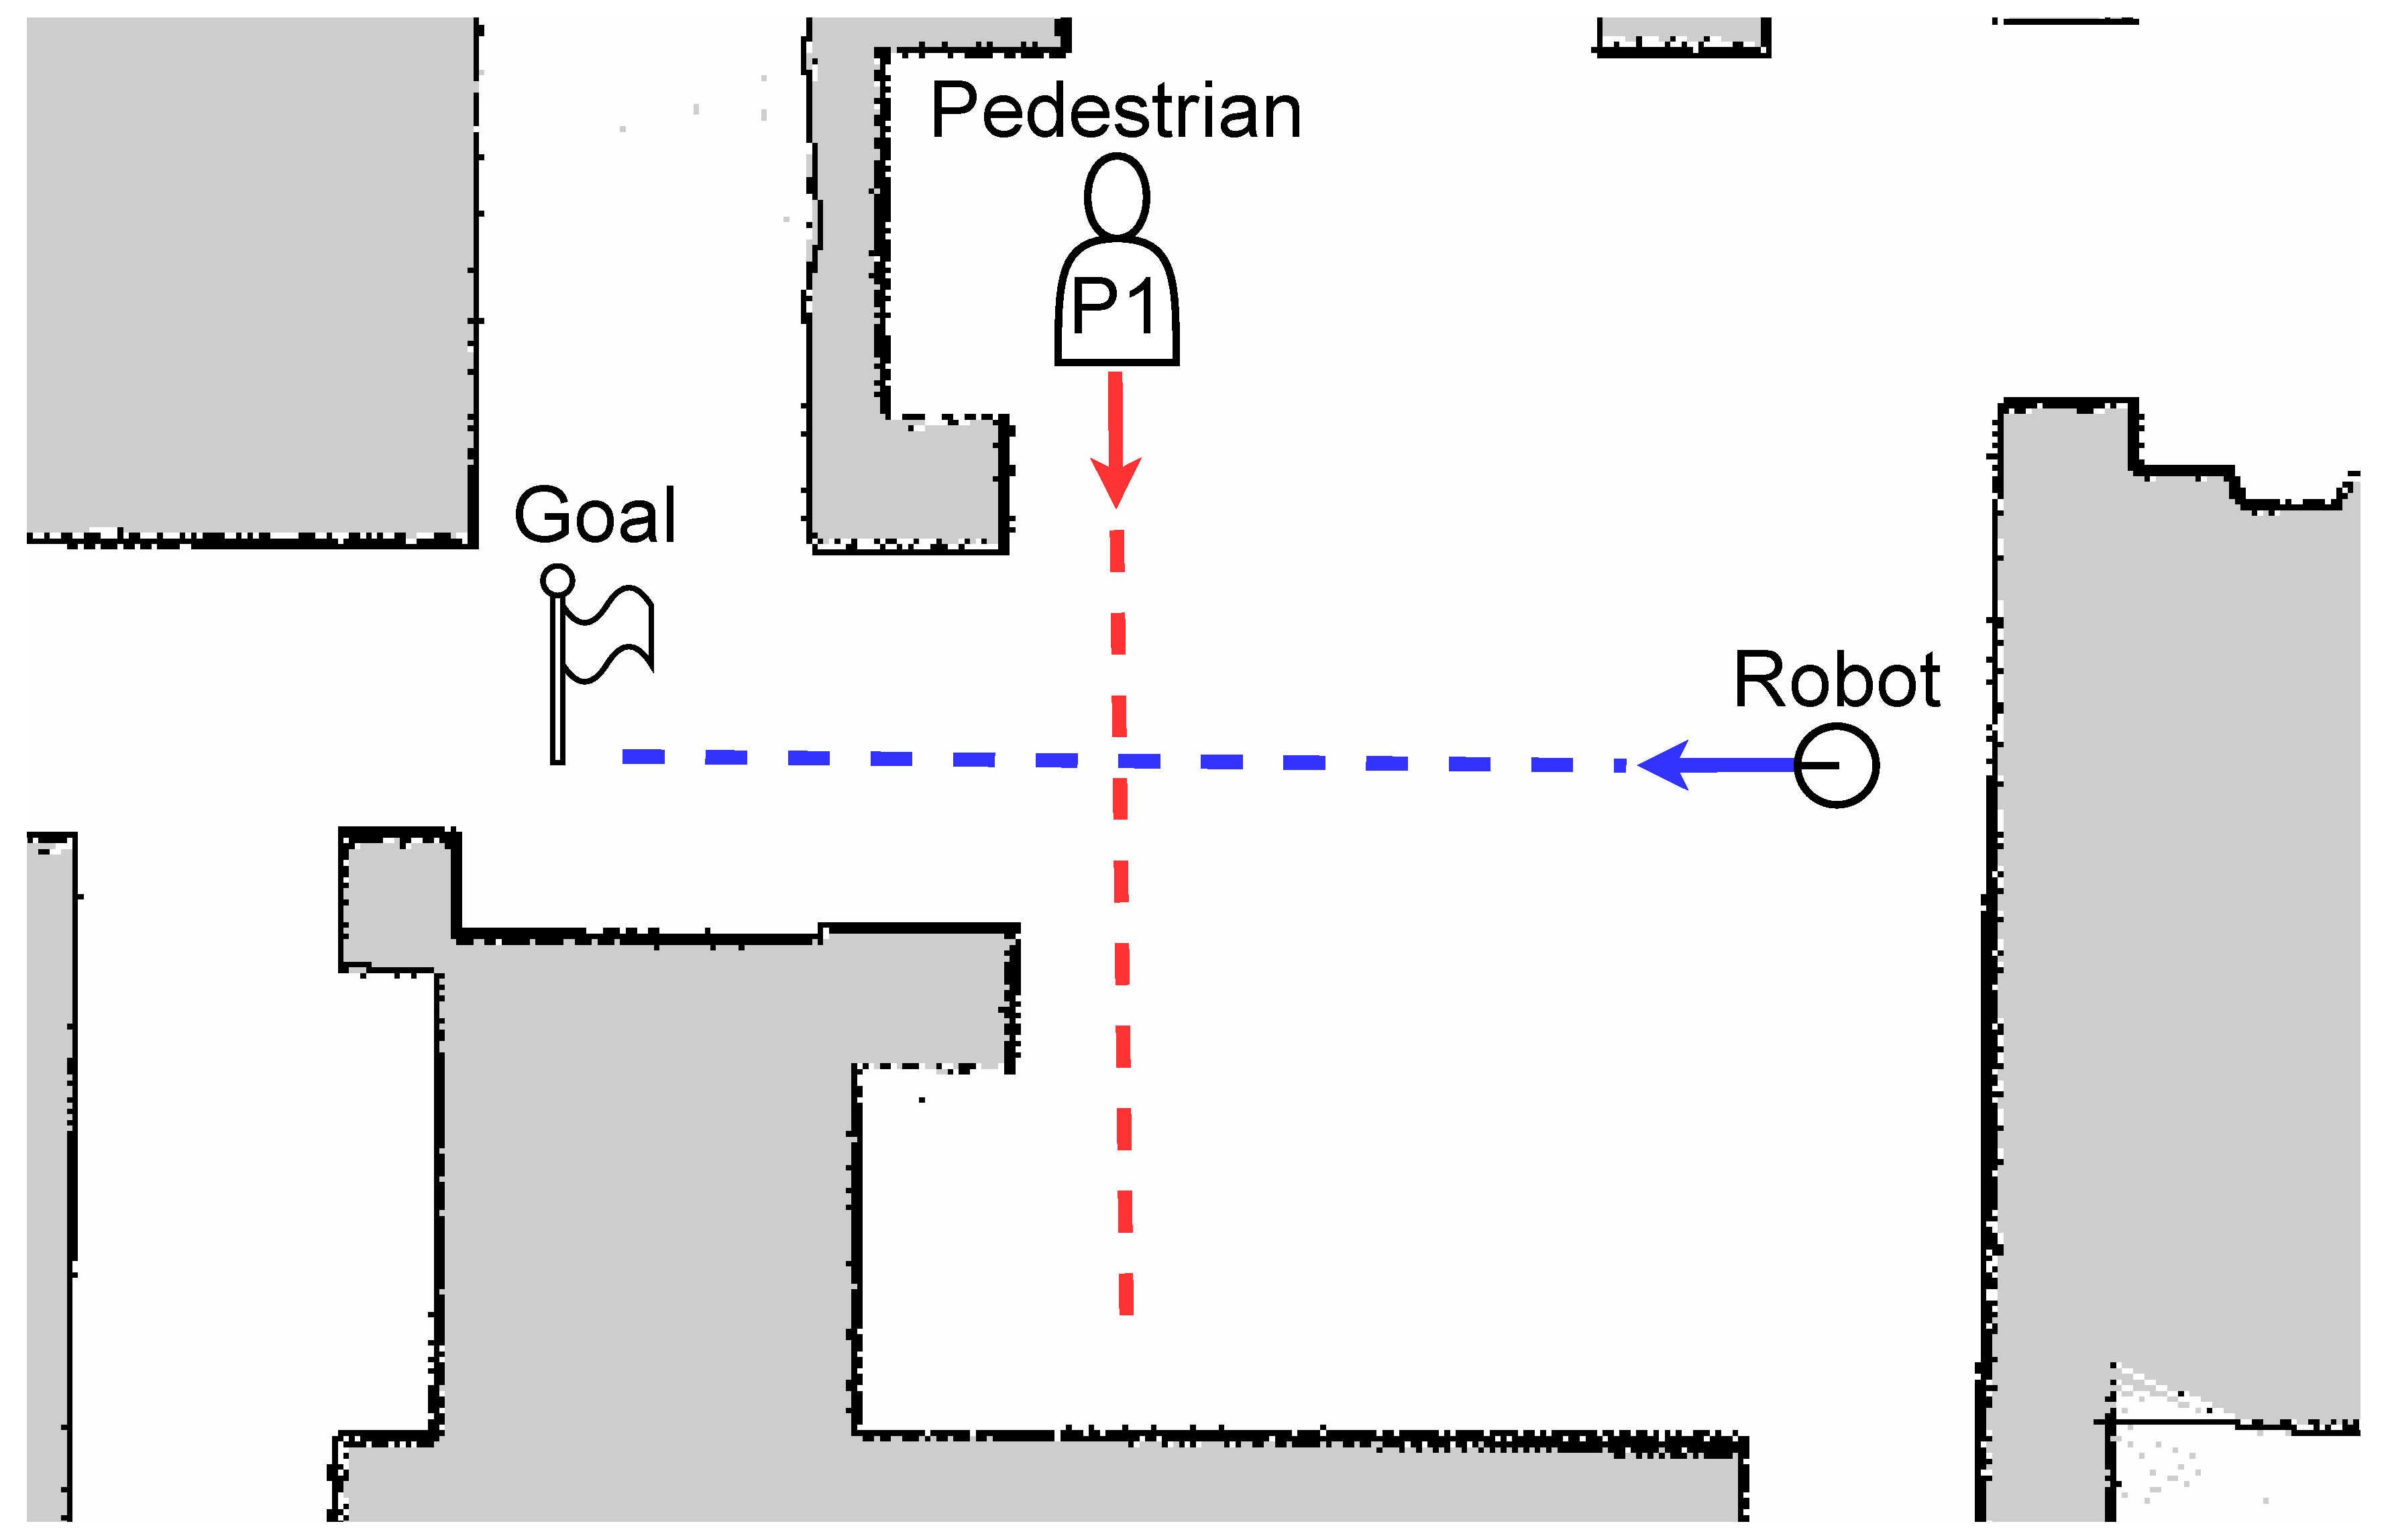
\includegraphics[keepaspectratio, scale=0.15]{images/scenario1.pdf}
    \caption{Scenario 1}
    \label{Fig:scenario1}
  \end{subfigure}
  \vspace{10pt}
  \begin{subfigure}{0.80\textwidth}
    \centering
    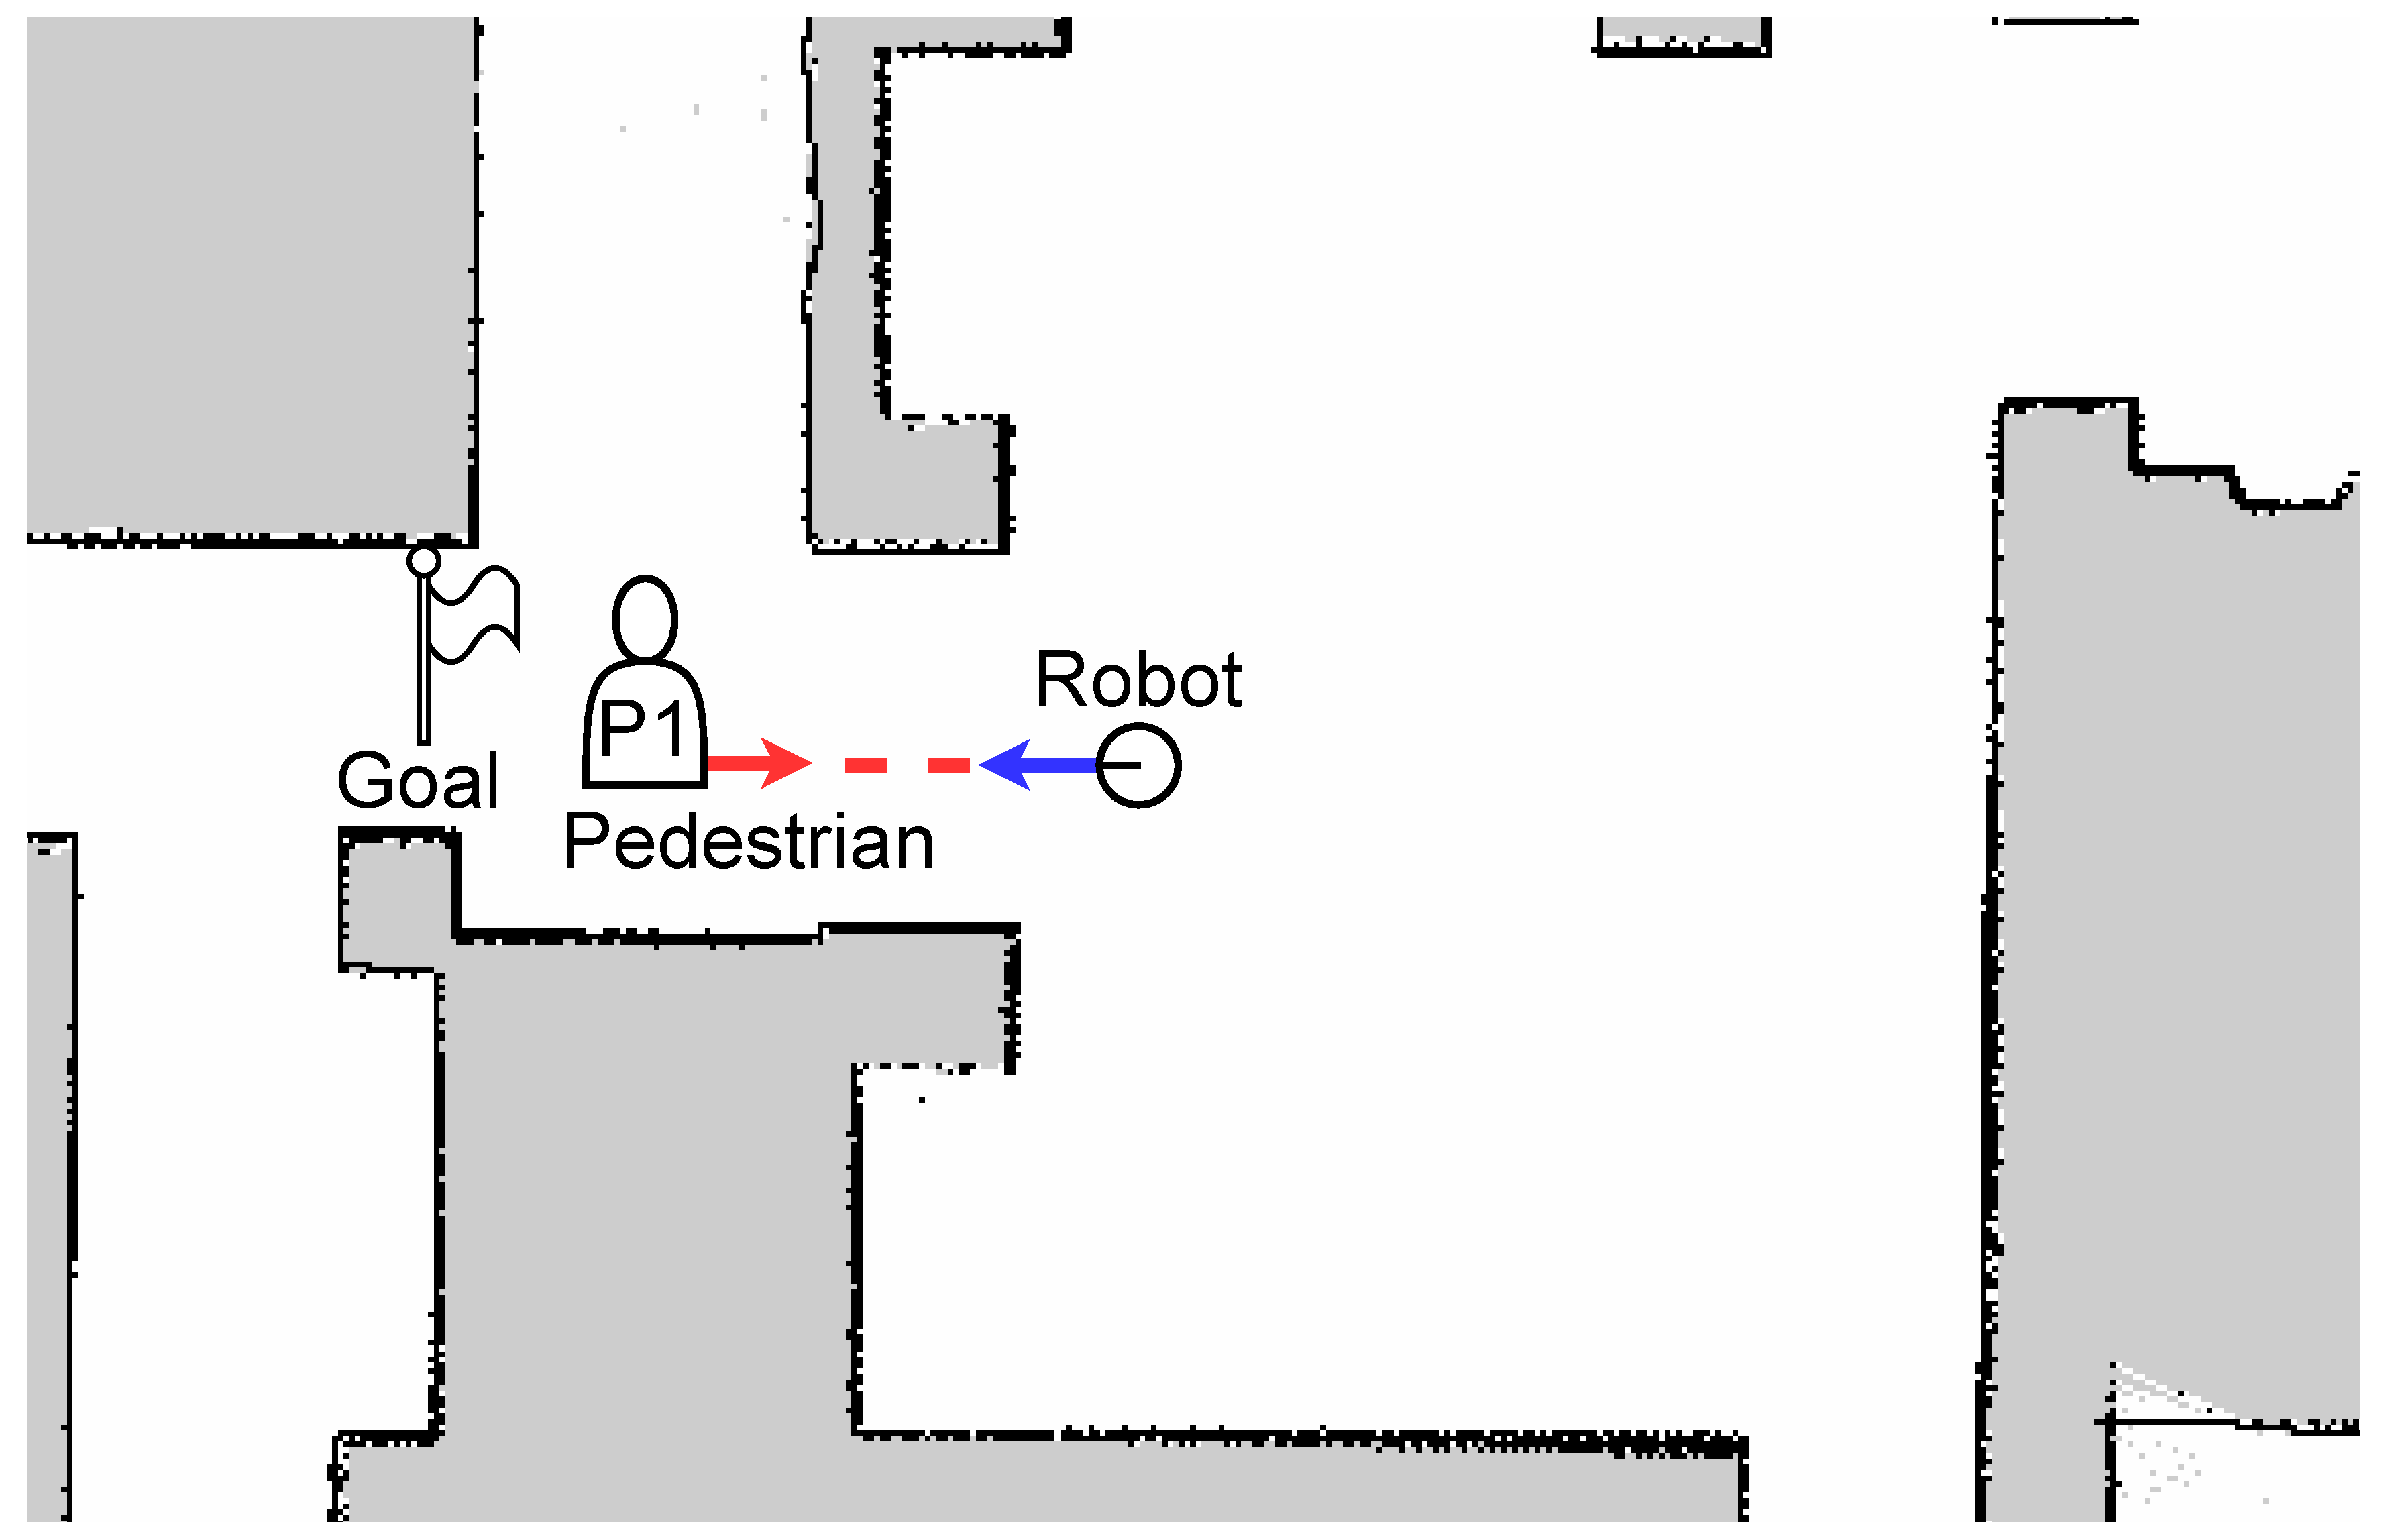
\includegraphics[keepaspectratio, scale=0.15]{images/scenario2.pdf}
    \caption{Scenario 2}
    \label{Fig:scenario2}
  \end{subfigure}
  \caption{Experiment Scenarios}
  \label{Fig:experiment-scenarios}
\end{figure}

\newpage

評価は以下の項目を基に行う.
\begin{itemize}
  \item 走行時間
  \item 走行距離
  \item 歩行者とロボット間の最小距離
  \item Time to Collision(TTC)
\end{itemize}

TTCは,ロボットと歩行者が衝突するまでの時間を示す指標であり,以下の式で計算される.

\begin{equation}
  \text{TTC} = \frac{d}{v}
\end{equation}

ここで,$d$はロボットと歩行者の距離,$v$はロボットの速度である.

\section{結果と考察}

\newpage
